\documentclass[12pt,a4paper,oneside]{article}
\usepackage[colorlinks=true, unicode]{hyperref}
\usepackage[utf8]{inputenc}
\usepackage[czech]{babel}
\usepackage{graphicx}
\usepackage{pdfpages}
\textwidth 16cm \textheight 25cm
\topmargin -1.3cm 
\oddsidemargin 0cm
\usepackage{footnote}
\pagestyle{empty}
\begin{document}
\title{Univerzální vstupní modul}
\author{Jakub Kákona, kaklik@mlab.cz}
\maketitle

\thispagestyle{empty}
\begin{abstract}
Vstupní modul s ochranou proti vysokému napětí. Může být použit v režimu se společnou zemí či s galvanickým oddělením. Je použitelný jak pro digitální, tak i pro analogové signály.
\end{abstract}

\begin{figure} [htbp]
\begin{center}
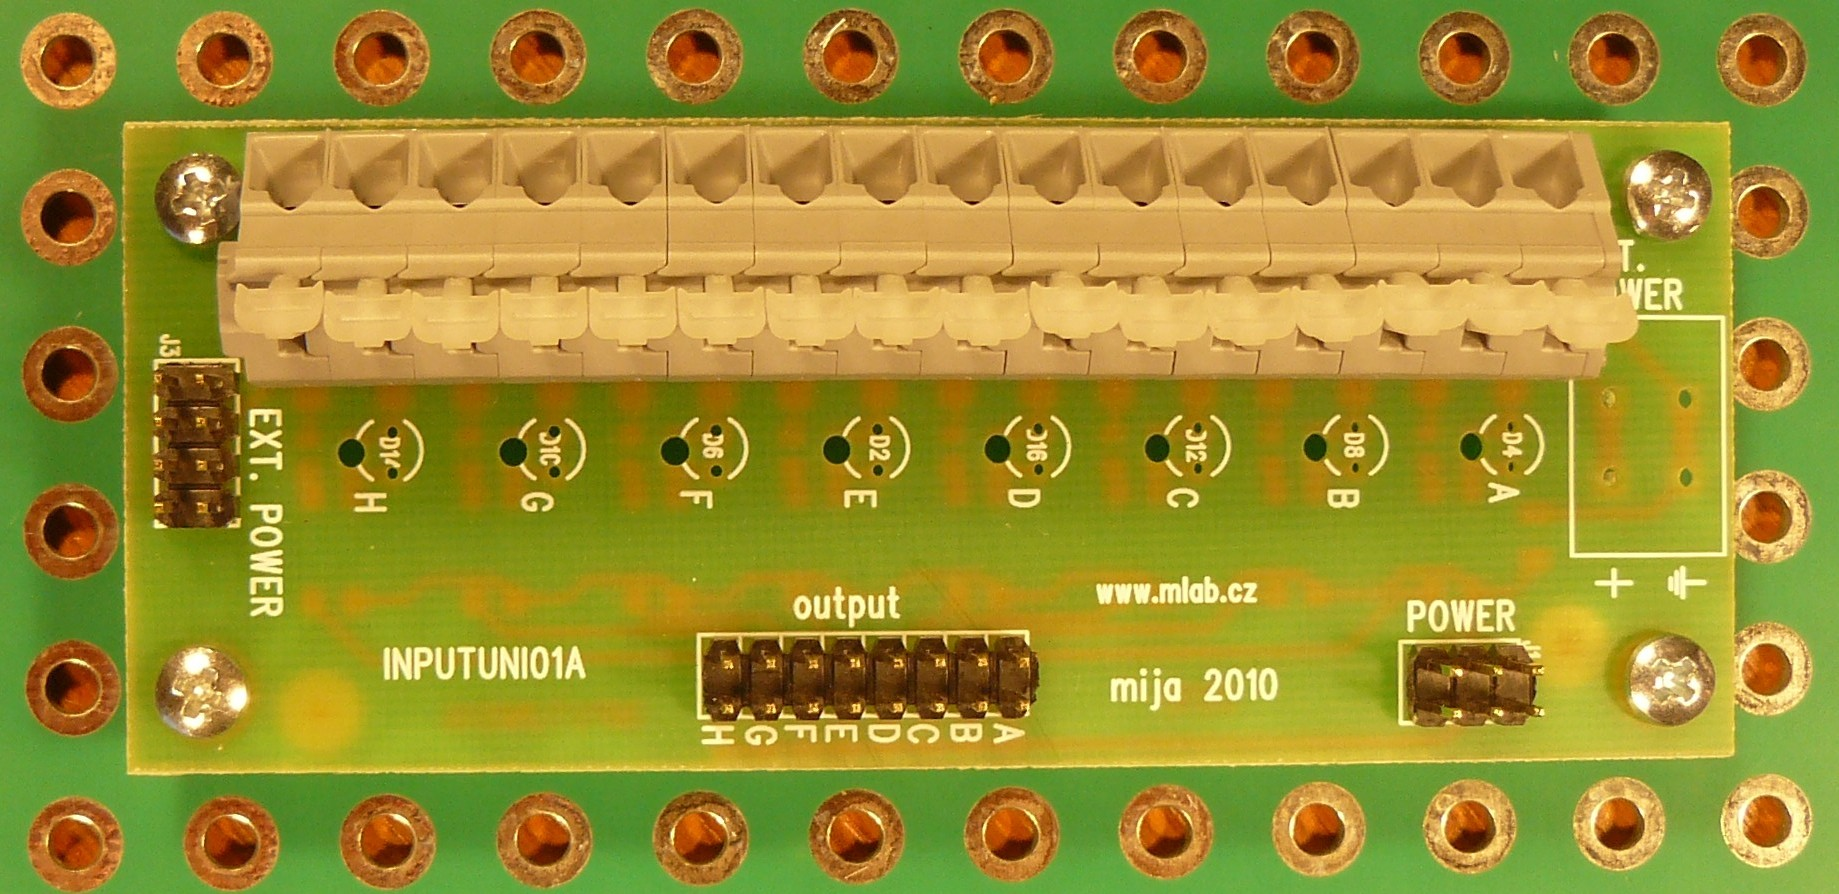
\includegraphics [width=100mm] {./img/INPUTUNI01A_Top_Big.jpg} 
\end{center}
\end{figure}

\begin{figure} [b]

\includegraphics [width=25mm] {./img/INPUTUNI01A_QRcode.png} 
\end{figure}

\newpage
\tableofcontents

\section{Technické parametry}
\begin{table}[htbp]
\begin{center}
\begin{tabular}{|c|c|p{4.7cm}|}
\hline
Parametr & Hodnota & Poznámka \\
\hline
Napájecí napětí Ext.POWER  & 5 až 12V & \\ 
\hline
\end{tabular}
\end{center}
\end{table}

\section{Popis konstrukce}

\subsection{Zapojení}

Modul konstrukčně umožňuje realizaci různých zapojení signálních vstupů.  Konkrétní volba zapojení je na znalostech konstruktéra.  Schéma modulu obsahuje pouze konstrukčně uvažované zapojení součástek. 

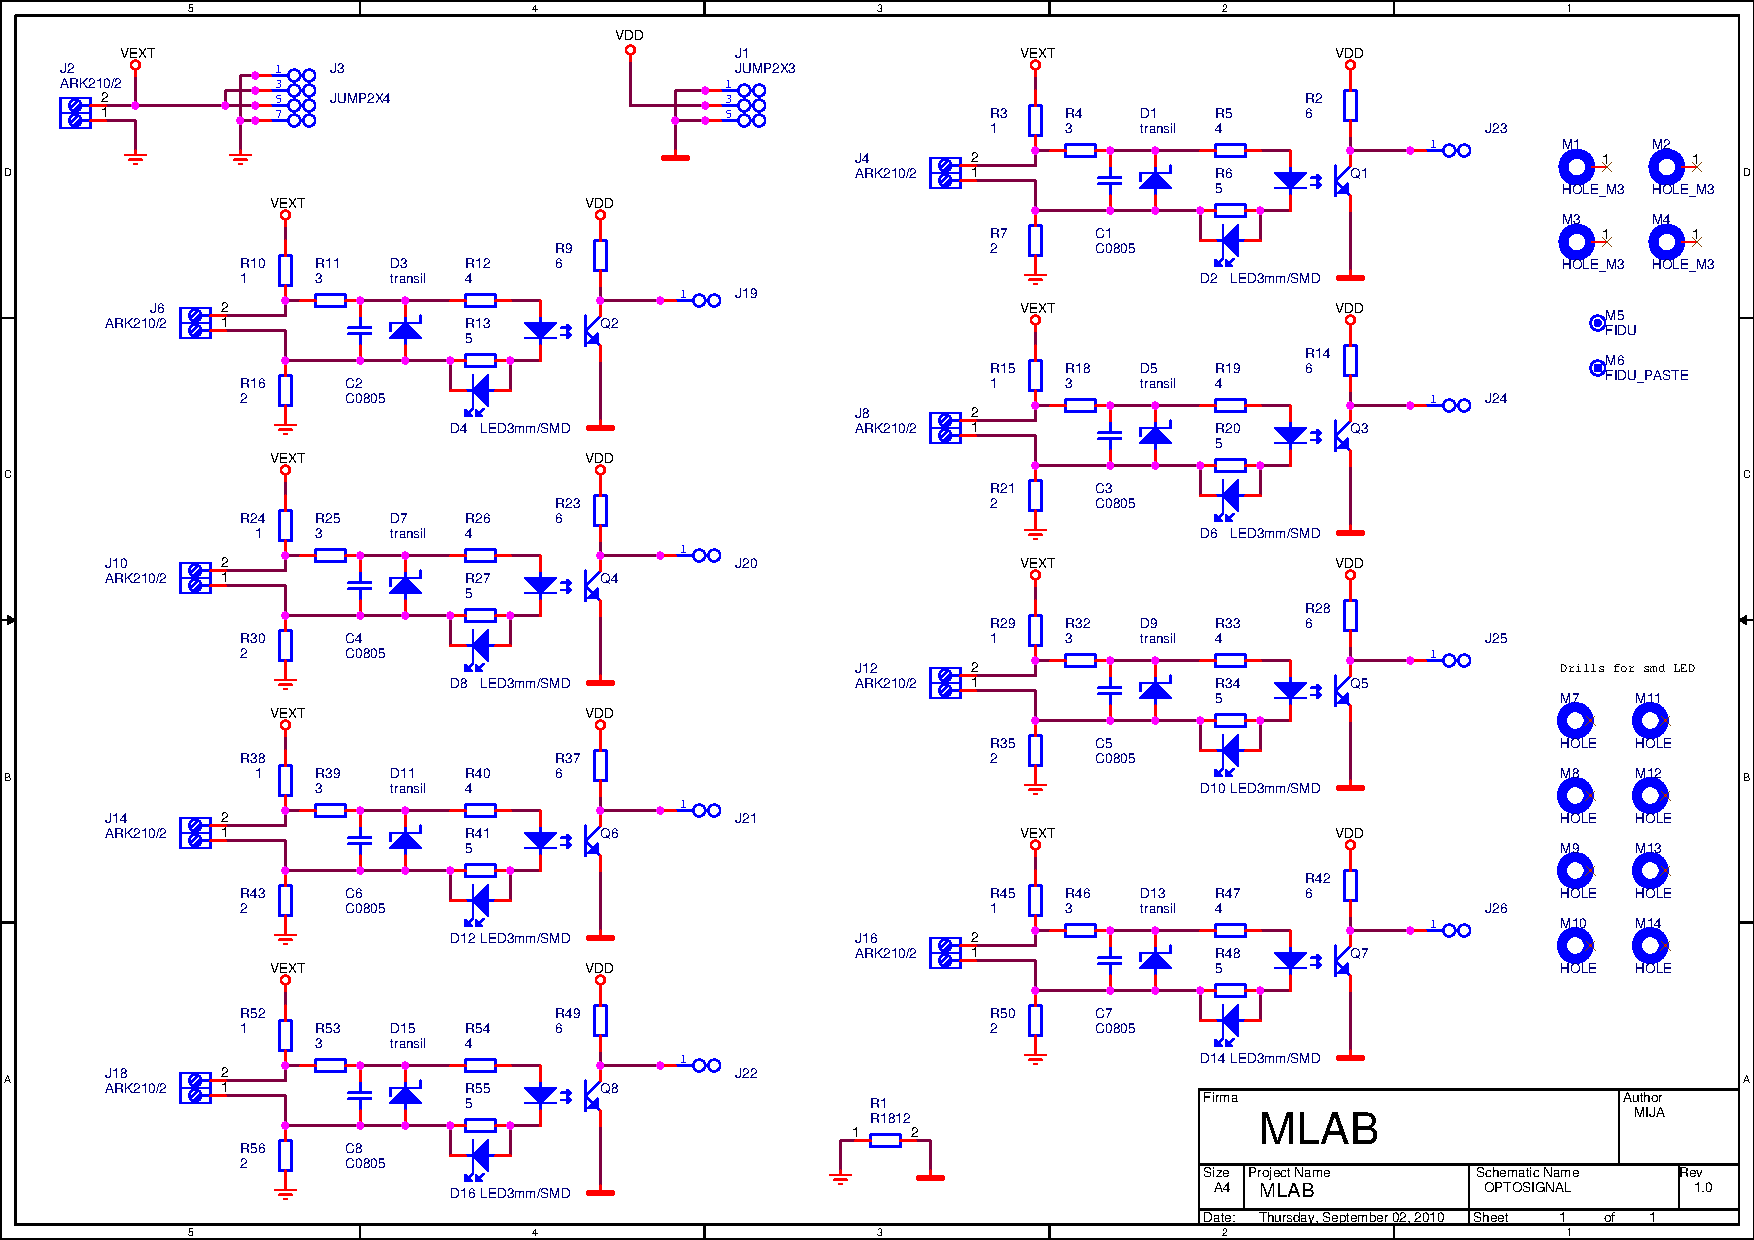
\includepdf[pages={1},landscape=true]{../../SCH/INPUTUNI.pdf}

\subsection{Mechanická konstrukce}

Modul klasicky předpokládá uchycení na čtyřech šroubech. Tento způsob uchycení může být problematický v případech, kdy hrozí časté vypojování a zapojování vodičů v prostřední části modulu. V takovém případě opora krajních šroubů proti základní desce nemusí být dostatečná a je vhodné modul dodatečně podložit například vytištěným plastovým dílem.  

\section{Výroba a testování}

Plošný spoj je navržen jak pro ruční pájení, tak i pro osazování pomocí pasty.  Modul se testuje optickou kontrolou spojů a následným připojením na laboratorní zdroj s omezením proudu.

\subsubsection{Osazení}

Modul je možné osadit i ručně. Rozložení součástek je na Obr. \ref{fig:osazovaci_plan}. Pozice vyhrazené pro součástky v pouzdru 0805 lze použít i vícenásobně, což znamená, že například kondenzátory a rezistory lze letovat na sebe. Toto řešení usnadňuje realizaci dolních propustí a dalších zapojení kde jsou využity paralelní RC obvody. 

\begin{figure} [h!tbp]
  \centering
  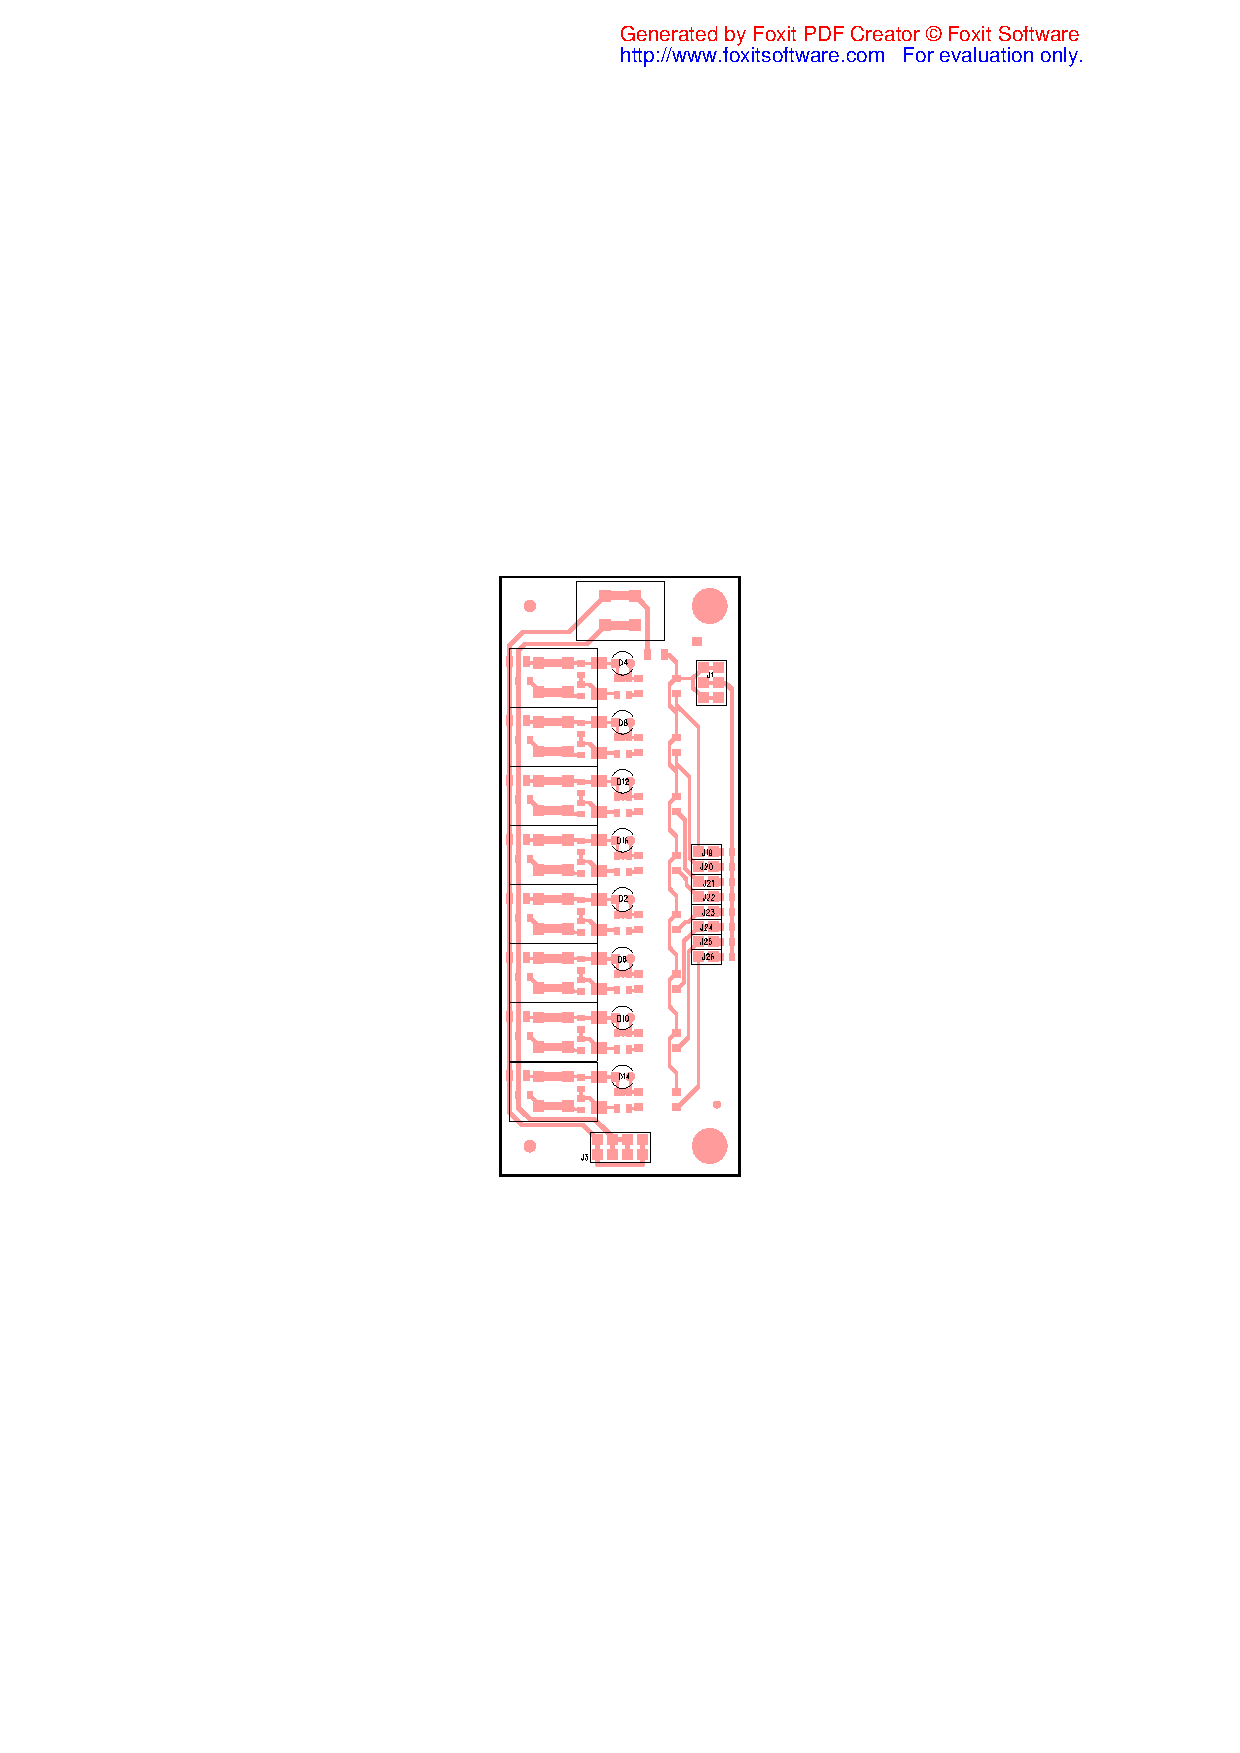
\includegraphics[trim = 8.0cm 9.5cm 8.0cm 9.5cm, clip, width=6cm]{../../CAM_DOC/O1.pdf}
  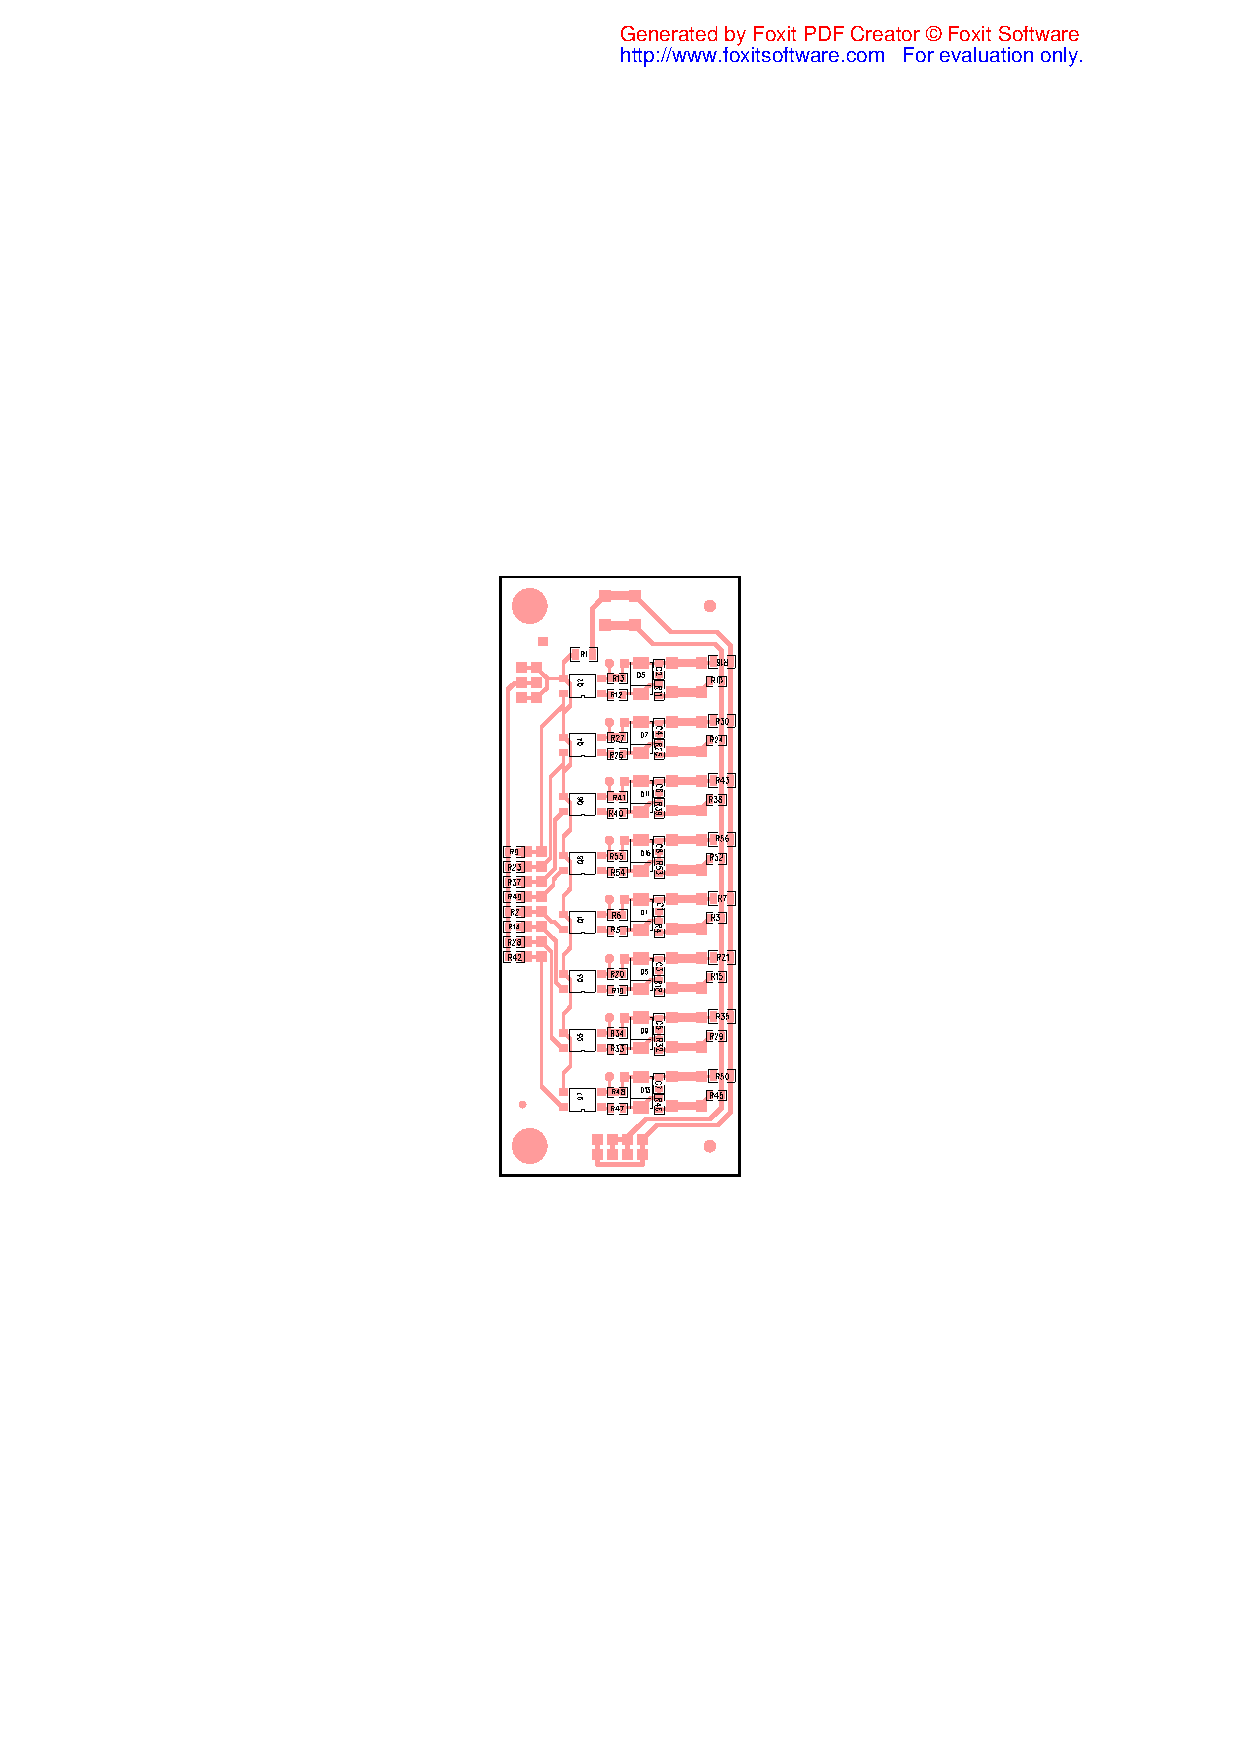
\includegraphics[trim = 8.0cm 9.5cm 8.0cm 9.5cm, clip, width=6cm]{../../CAM_DOC/O2.pdf}
  \caption{Osazovací plán horní a spodní strany plošného spoje}
  \label{fig:osazovaci_plan}
\end{figure}

Pro ukázku jsou zde uvedeny dvě základní možnosti osazení modulu. První varianta uvedená v tabulce \ref{seznam_soucastek_galvanic_isolation} je určena pro realizaci digitálního galvanicky odděleného vstupu. Takové zapojení je užitečné v případech, kde máme digitální signalizační signál vyvedený z nějakého průmyslového čidla. Ten má proto dobře definované logické úrovně, ale vzhledem k provoznímu prostředí na něm mohou být nebezpečné poruchy. Mikrokontrolér je potřeba před temito často vysokonapěťovými poruchami chránit a  k tomu slouží právě toto zapojení. 

Druhé možné zapojení v tabulce \ref{seznam_soucastek_switch} má podobné ochranné vlastnosti jako to předchozí, ale místo digitálního výstupu se na vstup připojuje mechanický spínač. Takový případ vyžaduje odlišné zapojení, protože je to pasivní signální prvek a navíc kontakty mechanického spínače musí být pro dobrý kontakt čištěny proudem.  K tomu slouží kapacita, která se nabíjí na napájecí napětí a při sepnutí spínače se vybije do odporů kontaktů, kde způsobí proudouvý náraz, který vede k velmi slabému natavení kontaktů a jejich lepšímu spojení.  Takovým způsobem pak k modulu lze připojovat i velmi masivní spínače určené pro výkonové aplikace, nebo standardní nástěnné světelné spínače. Minimální vhodná velikost kapacit osazených v modulu ale samozřejmě závisí na rozměrech kontaktů. Hodnota uvedená v tabulce je vyzkoušena pro běžný nástenný světelný spínač. 


\begin{savenotes}
\begin{table}[h!]
\begin{center}
\begin{tabular}{ |c|c|c|c| }
\hline 
Počet & Označení & Typ  & Pouzdro  \\ 
\hline 
8	&	-	&	C1,C2,C3,C4,C5,C6,C7,C8	&	C0805	\\
8	&	P6SMB13A	&	D1,D3,D5,D7,D9,D11,D13,D15	&	SMB	\\
8	&	LED3mm/SMD	&	D2,D4,D6,D8,D10,D12,D14,D16	&	LED3	\\
1	&	JUMP2X3	&	J1	&	JUMP2X3	\\
9	&	ARK210/2	&	J2,J4,J6,J8,J10,J12,J14,J16,J18	&	ARK210/2	\\
1	&	-	&	J3	&	JUMP2X4	\\
8	&	JUMP2X1	&	J19,J20,J21,J22,J23,J24,J25,J26	&	JUMP2X1	\\
8	&	LTV357T\_SMD	&	Q1,Q2,Q3,Q4,Q5,Q6,Q7,Q8	&	MFSOP6	\\
1	&	-	&	R1	&	R1206	\\
8	&	10k	&	R2,R9,R14,R23,R28,R37,R42,R49	&	R0805	\\
8	&	-	&	R3,R10,R15,R24,R29,R38,R45,R52	&	R0805	\\
8	&	10	&	R4,R11,R18,R25,R32,R39,R46,R53	&	R0805	\\
8	&	1k	&	R5,R12,R19,R26,R33,R40,R47,R54	&	R0805	\\
8	&	-	&	R6,R13,R20,R27,R34,R41,R48,R55	&	R0805	\\
8	&	-	&	R7,R16,R21,R30,R35,R43,R50,R56	&	R1206	\\
\hline 
\end{tabular}
\end{center}
\caption{Seznam součástek pro případ zapojení galvanicky odděleného digitálního vstupu.}
\label{seznam_soucastek_galvanic_isolation}
\end{table}
\end{savenotes}


\begin{savenotes}
\begin{table}[h!]
\begin{center}
\begin{tabular}{ |c|c|c|c| }
\hline 
Počet & Označení & Typ  & Pouzdro  \\ 
\hline 
8	&	470nF	&	C1,C2,C3,C4,C5,C6,C7,C8	&	C0805	\\
8	&	P6SMB13A	&	D1,D3,D5,D7,D9,D11,D13,D15	&	SMB	\\
8	&	LED3mm/SMD	&	D2,D4,D6,D8,D10,D12,D14,D16	&	LED3	\\
1	&	JUMP2X3	&	J1	&	JUMP2X3	\\
9	&	ARK210/2	&	J2,J4,J6,J8,J10,J12,J14,J16,J18	&	ARK210/2	\\
1	&	JUMP2X4	&	J3	&	JUMP2X4	\\
8	&	JUMP2X1	&	J19,J20,J21,J22,J23,J24,J25,J26	&	JUMP2X1	\\
8	&	LTV357T\_SMD	&	Q1,Q2,Q3,Q4,Q5,Q6,Q7,Q8	&	MFSOP6	\\
1	&	0R	&	R1206	&		\\
8	&	10k	&	R2,R9,R14,R23,R28,R37,R42,R49	&	R0805	\\
8	&	1k	&	R3,R10,R15,R24,R29,R38,R45,R52	&	R0805	\\
8	&	10	&	R4,R11,R18,R25,R32,R39,R46,R53	&	R0805	\\
8	&	1k	&	R5,R12,R19,R26,R33,R40,R47,R54	&	R0805	\\
8	&	-	&	R6,R13,R20,R27,R34,R41,R48,R55	&	R0805	\\
8	&	1k	&	R7,R16,R21,R30,R35,R43,R50,R56	&	R1206	\\
\hline 
\end{tabular}
\end{center}
\caption{Seznam součástek pro případ připojení mechanického spínače.}
\label{seznam_soucastek_switch}
\end{table}
\end{savenotes}



\begin{thebibliography}{99}

\end{thebibliography}
\end{document}